\section{Исследование и построение решения задачи}
\label{sec:Chapter3} \index{Chapter3}

Для того, чтобы внедрить наше решение в существующий проект по разработке компилятора MyTS,
сначала необходимо тщательно изучить его внутреннее устройство.
Составим обзор компонент фронтенда для понимания, как сделать наше решение качественной и логичной частью всего проекта.

\subsection{Исследование внутреннего устройства фронтенда}

\subsubsection{Лексер}

Этот компонент преобразует исходный код в последовательность токенов.
Входные данные должны быть корректной строкой UTF8.
Токены могут быть литералами, знаками препинания или ключевыми словами, представленными свойством \hl{Token::type}.
Поскольку JS содержит контекстуальные ключевые слова, например, \hl{static} - это ключевое слово внутри тела класса,
но в других местах это простой идентификатор, токены имеют дополнительное поле \hl{Token::keywordType},
которое всегда соответствует соответствующему ключевому слову независимо от реального \hl{Token::type}.
Поскольку на этом уровне могут возникать синтаксические ошибки, лексер может выдавать соответствующую ошибку.

\subsubsection{Область видимости}

Структуры \hl{binder::Scope} - это конструкции, в которых хранятся переменные.
Каждая область видимости имеет родителя - область по вложенности выше, все объявления \hl{binder::Decl},
которые хранятся в таблице переменных \hl{Scope::bindings}.
Эта таблица содержит строку в качестве ключа и переменную \hl{binder::Variable} в качестве значения.

\subsubsection{Объявления}

Объявления типа \hl{var a} или \hl{let b} во время синтаксического анализа преобразуются в \hl{binder::Decl}.
Каждое объявление знает имя и AST-узел, с которым оно связано.

\subsubsection{Переменные}

Переменные по умолчанию не создаются.
Декларации преобразуются в переменные, если они проходят проверку в рамках области видимости.
Структура переменной \hl{binder::Variable} содержит в себе объявление, из которого она взята, а также имеет
\hl{checker::Type}, который будет представлять фактический статический тип переменной.
Этот тип неизвестен во время синтаксического анализа и заполняется позже компонентом \hl{Checker}.

\subsubsection{Binder}

Этот компонент создает и проверяет все привязки(bindings) деклараций к области видимости.
Сам по себе он не является отдельным анализом.
Каждая проверка привязки запускается в процессе синтаксического анализа.
В настоящее время триггерами могут быть:

\begin{itemize}[left=2em]
    \item Создание новой области видимости.
    \item Добавление объявления в текущую область видимости.
    Если она не может добавить привязку, возникает синтаксическая ошибка.
\end{itemize}

\subsubsection{Парсер}

Парсер является одним из основных компонент и взаимодействует с binder-ом и лексером одновременно.
Синтаксический анализ является однопоточным, и входные данные обрабатываются только один раз.
Для парсинга выбран синтаксический анализатор LR(1), поэтому он видит только следующий токен,
но может заглянуть в следующую точку кода.
Однако из-за новых возможностей стандарта ES2015 список параметров лямбда функций и шаблоны деструктурирования
больше не могут быть корректно прочитаны, заглядывая только на один токен вперед.
В этих сценариях синтаксический анализатор работает в отказоустойчивом режиме, что означает,
что он следует менее строгой грамматике, чем стандартная.
Всякий раз, когда закрывающий токен для этих языковых элементов найден или не найден, выполняется обход построенного AST
дерева и проверка его правильности в соответствии с правилами грамматики.
По мере того как AST строится во время синтаксического анализа, также создается дерево областей видимости.
Как только парсер обрабатывает очередной блок кода или функцию, запускается binder, который создает для них новую область
видимости и привязывает их к ней.
Поскольку время жизни этих областей совпадает со временем жизни соответствующих узлов AST дерева,
структуры представляющие узел также сохраняют у себя эти области видимости.
Всякий раз, когда считано объявление переменной, запускается binder для проверки привязки.
Таким образом, в общем случае синтаксический анализатор уведомляет binder только о том, что он обнаружил
новое начало области видимости или объявление новой переменной.

\subsubsection{AST дерево}

ASTNode - это базовый класс всех узлов, сгенерированных парсером.
Узел AST хранит в себе данные о позиции в исходном коде, родительский узел и другие атрибуты,
которые добавляются дочерним классам при наследовании.

\subsubsection{Анализ имен переменных}

После того, как исходный код обработан парсером, AST проходит анализ имен переменных.
После него создается класс программы, содержащий AST дерево, позиции переменных в исходном коде и некоторые метаданные.
Главной целью этого анализа является определение типа переменной для обеспечения эффективной многопоточной компиляции
без блокировки, не считая планирования потоков.
Переменная может быть локальная или лексическая.
Во время обхода AST дерева мы ссылаемся на уже сгенерированные области видимости, присвоенные statement узлам,
чтобы определить, в какой области мы на самом деле находимся.
Всякий раз, когда мы оказываемся в узле идентификатора переменной \hl{ir::Identifier},
анализатор пытается разрешить ее тип из текущей области.
Если у переменной нет конфликтов с какой-либо другой переменной из области видимости \hl{binder::VariableScope}
(чаще всего это \hl{binder::FunctionScope}, иногда \hl{binder::LoopScope}), переменная объявляется как локальная.
В противном случае она получает лексический индекс из ближайшей области видимости и помечается как лексическая.
Каждый раз, когда из области видимости запрашивается лексический слот на переменную, область становится лексической.
Это означает, что во время компиляции в начале функции должно быть создано так называемое лексическое окружение.
В этом анализе мы также определяем, является ли локальная переменная внутри объявления цикла частью замыкания
внутри его тела.
Результат этого анализа определяет, должны ли цикл или его декларация быть лексическими или нет.
Таким образом, перед переходом непосредственно на стадию кодогенерации AST обрабатывается только один раз.
Каждая область видимости содержит в себе информацию о том, нуждается ли она в лексическом окружении или нет,
и каждая переменная знает, является ли она лексической или нет.

\subsubsection{Чекер}

Этот компонент семантически анализирует код, используя AST дерево, области видимости и переменные.
Чекер обходит AST дерево и проверяет каждый узел, используя виртуальную функцию \hl{Checker},
перегруженную для всех узлов по-своему.
Когда чекер обнаруживает узел с объявлением какой-то переменной, он выполняет ее поиск во всех областях видимости
по степени их вложенности друг в друга.
Как только найдено объявление этой переменной в какой-то области видимости, чекер присваивает тип выражения к узлу
дерева, если он задан явно, либо использует для этого вывод типов.

\begin{itemize}[left=2em]
    \item При незаданной аннотации, тип объявленной переменной выводится с помощью инициализатора.
    \item При объявлении функции чекер создает для нее сигнатуру, которая состоит из параметров в заданном порядке
    и типа возвращаемого значения.
    Оно в свою очередь выводится из явно указанной аннотации типа или выражения, следующего за return в теле функции.
    \item При объявлении интерфейса чекер создает объектный тип, который хранит в себе все поля и их типы, а также
    сигнатуры методов и конструкторов интерфейса.
    \item При объявлении псевдонима типа чекер использует тип, который этому псевдониму и присваивается.
\end{itemize}

\subsubsection{TsType}

Как только тип объявления вычислен, ему присваивается значение ts-типа объявленной переменной.
Используя структуру \hl{checker::Type}, чекер может проверять на валидность выражения присваивания, бинарные или унарные
операции, вызовы функций и конструкторов, доступы к полям класса и наследование.
Важно отметить, что statement не создает тип, это делают только выражения.

\begin{itemize}[left=2em]
    \item Statement проверяется только семантически.
    Например, если statement проверяется на наличие у него выражения-условия,
    которое вычисляется в тип void, то чекер сообщает об ошибке, поскольку выражения типа void не могут быть
    проверены на истинность.
    \item Выражения, с другой стороны, по своей сути порождают типы.
    Например, бинарное выражение \hl{5 + 6} порождает числовой тип.
    Вот почему функция \hl{ASTNode::Check} узла statement всегда возвращает значение nullptr, а функция \hl{ASTNode::Check} узла
    выражения всегда возвращает тип, созданный этим выражением.
\end{itemize}

\subsubsection{Отношения}

В определенный момент во время семантического анализа чекер должен соотнести различные типы друг с другом.
Например, если переменной присвоено значение a = 15, чекер сравнивает тип переменной a с типом
инициализатора, который представляет собой числовое литеральное выражение, приводимое к числовому типу.
Если a был объявлен как \hl{let a: string}, то это присвоение приведет к ошибке, поскольку тип string не может быть
присвоен типу number.
В зависимости от операции, используемой с переменными, существует 3 различных отношения типов:

\begin{itemize}[left=2em]
    \item Отношение идентичности: отношение является истинным, если два сравниваемых типа абсолютно идентичны.
    Оно используется при повторном объявлении переменной или поля, и это наиболее сильное отношение.
    \item Отношение присваивания: отношение является истинным, если тип с правой стороны может быть присваивоен типу
    с левой стороны.
    Оно используется при обработке присваиваний, операндов бинарных выражений, наследования (отношение базового и дочернего класса),
    а также для проверки совместимости типа возвращаемых выражений из return с типом возвращаемого значения, объявленного в функциях.
    \item Отношение приводимости: отношение является истинным, если тип в правой части может быть приведен к типу в левой части.
    Оно используется при работе с операторами сравнения, приведения типов и в не сильно отличается от отношения присваивания.
    Это самое слабое отношение.
\end{itemize}

\subsubsection{Сигнатуры функций}

Сигнатуры создаются для функций и методов, и они могут быть явно объявлены в теле интерфейса или класса,
используя следующий синтаксис: \hl{(a: number, b: string): number}.
Существует два типа сигнатур: сигнатуры функций и конструкторов.
Сигнатуры функций используются для проверки правильности вызовов функций.
Например, если объявление функции с именем func1 было объявлено с сигнатурой (a: string, b: string), то оно не может
быть вызвано с меньшим или большим количеством параметров, чем 2, и аргументы вызова функции должны быть присваиваемы
типу параметра сигнатуры в правильном порядке.
Таким образом, чекер выдаст ошибку в любом из этих случаев:
func1(1), func1(1, 2, 3), func1("foo"), func1(2, "bar").
Сигнатуры конструкторов идентичны по своим правилам.
Разница лишь в том, что они используются при создании объектов и, соответсвенно, в выражения с ключевым словом new.

\subsubsection{Lowering фазы}

Lowering преобразование - это фаза трансформаций, работающая после чекера и перед кодогенерацией,
во время которой происходит обход AST дерева, преобразуя некоторые его узлы и заменяя отфильтрованные выражения более
простыми и низкоуровневыми конструкциями.
Стоит уточнить, что не все фазы lowering-а проходят после чекера.
На самом деле, некоторые проходы трансформируют AST дерево и до семантического анализа.
У каждого lowering прохода имеются предусловие и постусловие.
Как видно из названий, предусловие является триггером для запуска трансформации дерева для конкретного узла, а
постусловие проверяет, что преобразование было успешным и не нарушило структуру и инварианты AST дерева.
Преимущества внедрения lowering проходов перед кодогенерацией следующие:

\begin{itemize}[left=2em]
    \item Абстрагирует код – различные lowering фазы могут быть написаны независимо друг от друга
    \item Упрощает кодогенерацию
    \item Легкость отладки.
    Дает возможность распечатать и проанализировать состояние AST дерева до и после какой-то определенной трасформации.
\end{itemize}

Недостатки lowering проходов:

\begin{itemize}[left=2em]
    \item Увеличение времени компиляции
    \item Возможная утеря отладочной информации
    \item Основательный семантический анализ проводится до большинства lowering проходов.
    После трансформаций не исключено, что состояние AST дерева станет некорректным.
    \item Подходит только для некоторых задач
\end{itemize}

Примеры lowering фаз, которые осуществляют трансформацию определенных конструкций языка и AST дерева:

\begin{itemize}[left=2em]
    \item Обработка лямбда-функций, генерация для них объекта.
    \item Раскрытие объектных литералов
    \item Боксинг и анбоксинг переменных
    \item Преобразование выражений в вызовы рантайм функций
    \item Оптимизации
\end{itemize}

\subsubsection{Кодогенерация из промежуточного представления}

Кодогенерация осуществляется параллельно для каждого AST узла.
Класс \hl{Gen} контролирует все функции, которые генерируют байткод или управляют ресурсами.

\subsubsection{Аллокация регистров}

Формат исполняемого файла требует, чтобы все параметры размещались в конце локальных регистров.
Поскольку в данном языке есть инициализация полей и переменных по умолчанию, а также rest параметры, от локальных
регистров требуется выполнение определенных стандартных действий.
Для этого нам нужно загружать соответствующие параметры в регистры.
Номер соответствующего регистра зависит от количества используемых локальных регистров, что является циклической
зависимостью.
Для разрешения этой проблемы, была представлена следующая структура регистра:

\begin{table}[h]
    \centering
    \begin{tabular}{|c|c|c|c|c|c|}
        \hline
        локальный n & локальный 1 & локальный 0 & параметр 0 & параметр 1 & параметр n \\
        \hline
        ... & 65534 & 65535 & 65536 & 65537 & ... \\
        \hline
    \end{tabular}
\end{table}

Таким образом, во время генерации кода выделяемые регистры располагаются в порядке убывания, и при
необходимости все spill-fill инструкции генерируются сразу в нужном месте.
Как только вся кодогенерация завершена, становится известно количество всех выделенных локальных регистров, а аргументы
генерируемых инструкций преобразуются следующим образом:

\begin{itemize}[left=2em]
    \item Локальные регистры отображаются в диапазоне uint16\_t
    \item Параметры вычисляются как UINT16\_MAX - общее количество регистров.
\end{itemize}

\subsubsection{Выделение регистров для локальных переменных при кодогенерации}

Каждый раз, когда очередной шаг кодогенерации попадает в область видимости блока или функции, класс \hl{Gen}
обрабатывает локальные переменные.
На этом этапе известно, является ли переменная лексической или локальной.
Лексические переменные не затрагиваются, поскольку они уже получили свой лексический индекс во время
анализа имен переменных.
Поскольку индекс регистра, в котором лежит локальная переменная, считывается или записывается только классом \hl{Gen},
присваивание регистра на этом этапе безопасно.
Всякий раз, когда область видимости заканчивается, эти регистры освобождаются и могут быть повторно
использованы позже.

\subsubsection{Разрешение имен переменных}

При генерации байткода всякий раз, когда требуется разрешить имя переменной \hl{ir::Identifier},
мы используем тот же метод, что и при анализе имен переменных:
начинаем поиск имени переменной из текущей области и отслеживаем, сколько областей видимости мы проходим.
В зависимости от результатов поиска принимается решение, какой байткод нам нужно сгенерировать для разрешения:

\begin{itemize}[left=2em]
    \item Местных
    \item Лексических
    \item Модульных
    \item Глобальных
\end{itemize}

переменных.
На данный момент информация о типе переменной, вычисленной чекером, уже доступна, но в данный момент
не используется.

\subsubsection{Узел промежуточного представления}

Узел промежуточного представления имеет класс \hl{IRNode}.
Каждая инструкция из архитектуры набора команд (ISA), сгенерированная из файла isa.yml, имеет свой класс,
который содержит только необходимые операнды.
Исключением является ассемблерный класс \hl{Ins}, который содержит список операндов каждого типа.
Этими типами операндов могут быть:

\begin{itemize}[left=2em]
    \item Виртуальный регистр - VReg
    \item Иммидиат - Imm
    \item Строка - StringView
    \item Метка - Label
\end{itemize}

Кроме того, их каждый узел промежуточного представления содержит в себе узел AST дерева,
чтобы получать информацию о позиции какой-либо сущности в исходном коде для генерации отладочной информации.
В конце каждой кодогенерации узлы \hl{IRNode} будут преобразованы в ассемблерные инструкции \hl{Ins}.
Во время преобразования:

\begin{itemize}[left=2em]
    \item Сохраняются строковые операнды, которые позже будут добавлены в таблицу строк сгенерированной программы
    \item Операнды VReg переназначаются на их реальные регистровые индексы.
\end{itemize}

\subsubsection{Эмиттер}

Этот компонент преобразует каждый шаг кодогенерации из класса \hl{Gen} в ассемблерный класс \hl{Function}.
Список сущностей, которые преобразуются в ассемблер:

\begin{itemize}[left=2em]
    \item Метки
    \item Try-catch блоки
    \item Инструкции
    \item Отладочная информация
\end{itemize}

Также сохраняются все общеиспользуемые данные в класс \hl{ProgramElement}, находящийся во фронтенде.
Такими данными могут быть, например, строки и литералы, которые позже записываются в ассемблерный класс \hl{Program}.
Всякий раз, когда генерируется класс \hl{Gen}, эмиттер объединяет все элементы программы промежуточного представления
\hl{ProgramElement} и заполняет таблицу функций уже созданными ассемблерными классами \hl{Function}.

\subsection{Схематичное устройство компилятора}

Кратко проанализировав и описав выше основные компоненты фронтенда, которые позволяют трансформировать исходный код на
языке MyTS в ассемблерное представление \hl{Program} с дальнейшей оптимизацией и генерацией байткода,
стоит представить обобщенную схему работы данного компилятора:

\begin{figure}[h]
    \centering
    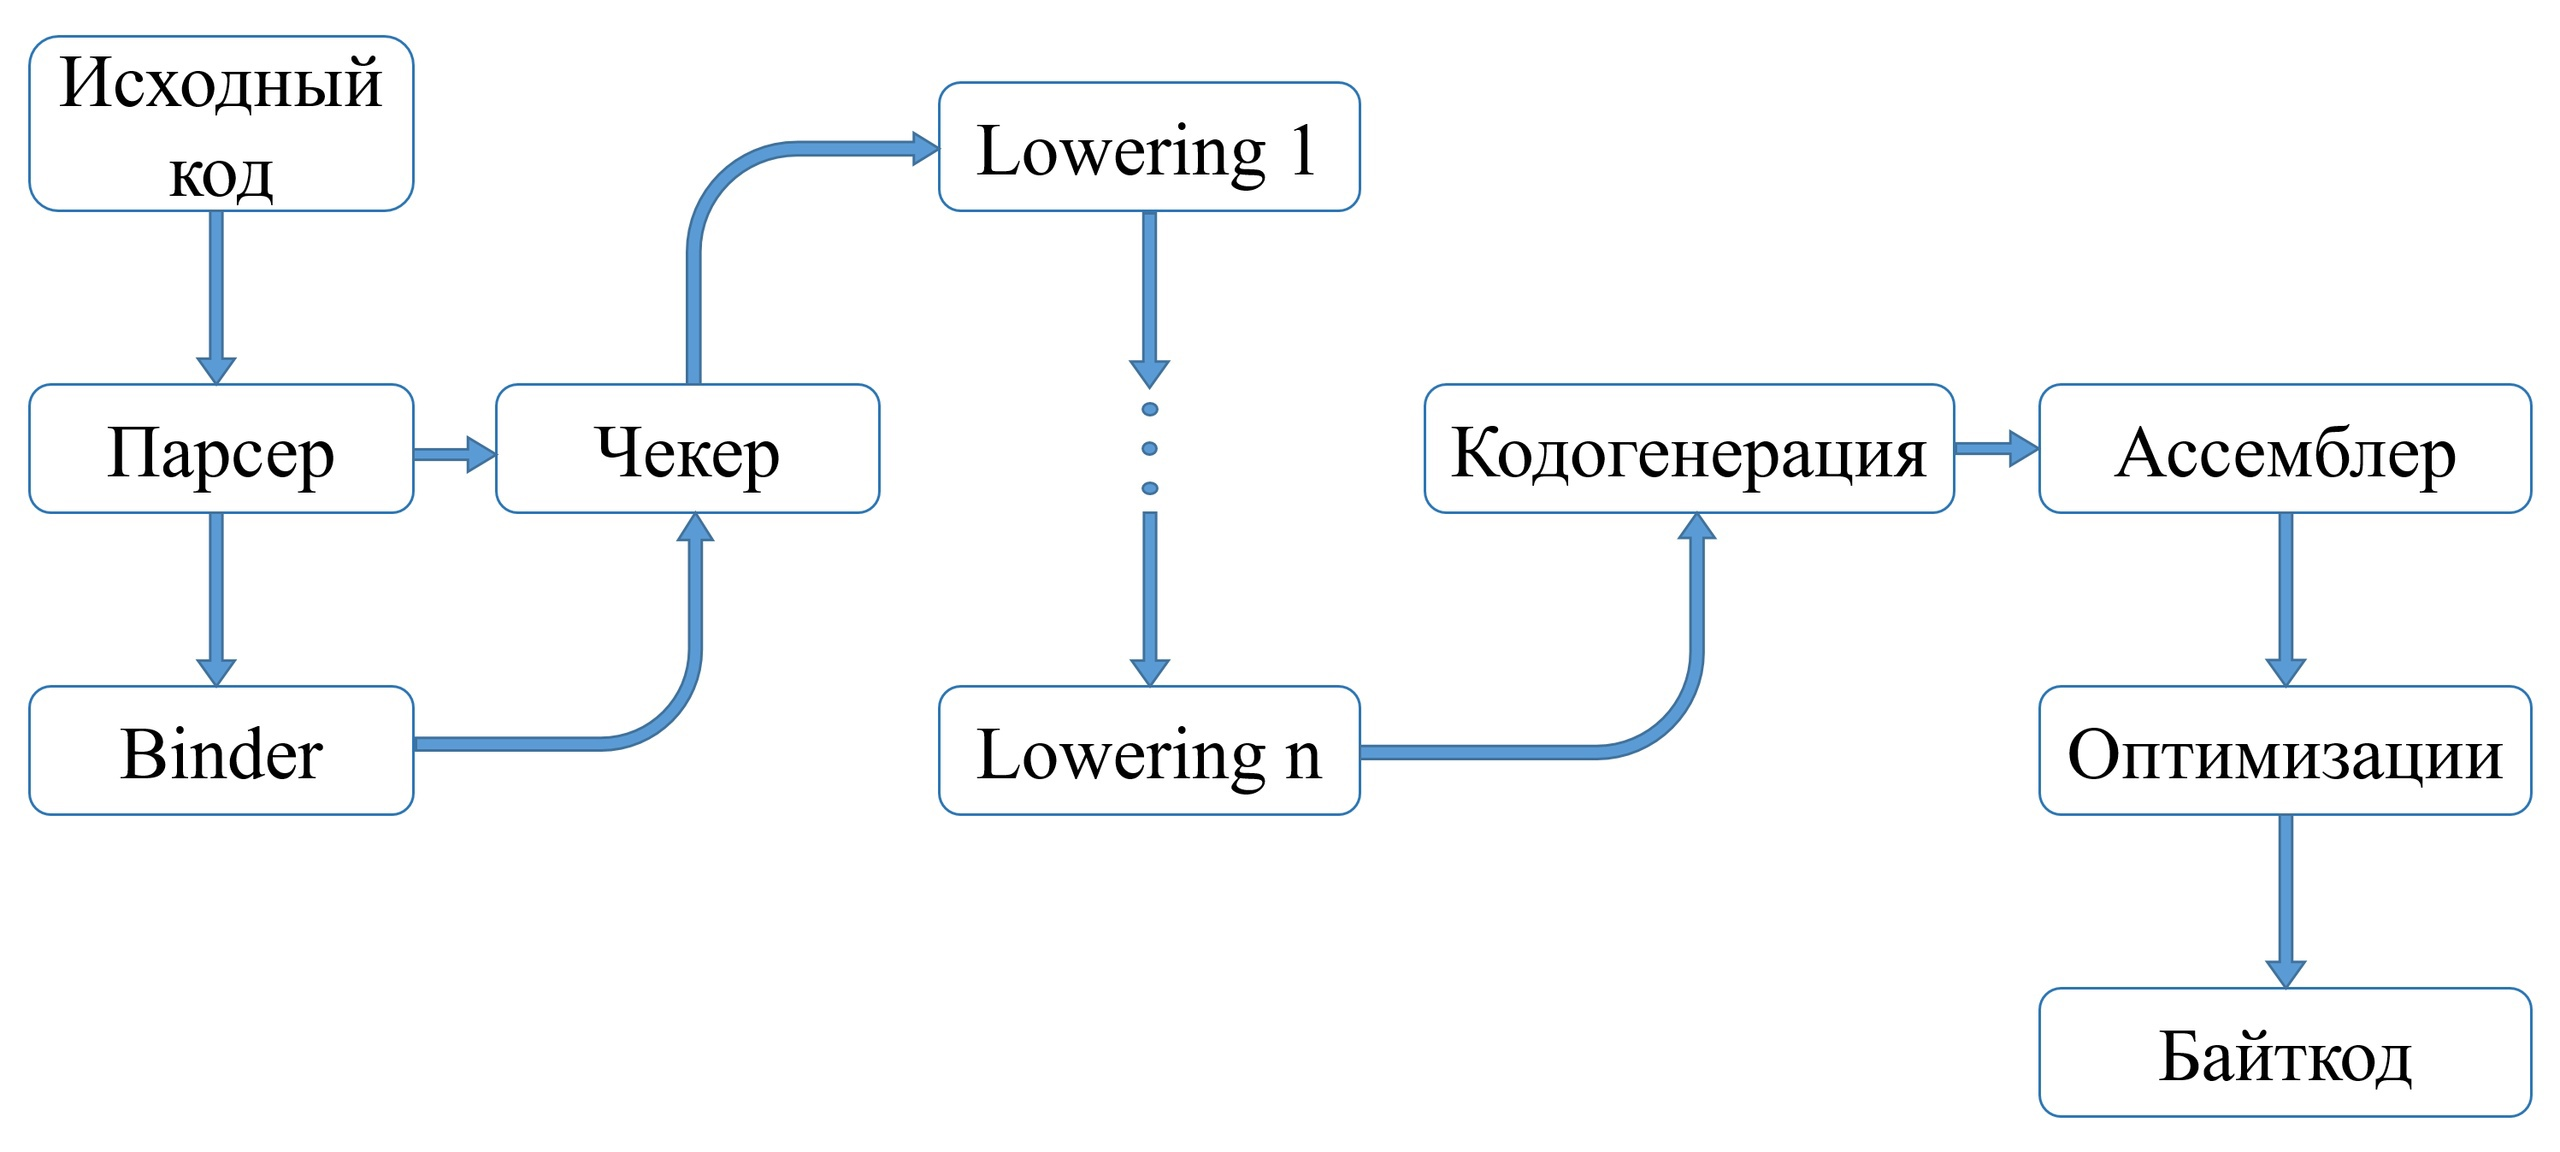
\includegraphics[scale=0.18]{Lowering1.jpg}
    \caption{Схема работы компилятора}\label{fig:figure}
\end{figure}

todo: описать боксинг анбоксинг

\newpage
